\chapter{Design}\label{chap:Design}

This section goes over the initial design for the solution we present. Any major deviations from this design are noted in Chapter~\ref{chap:Implementation}. To make design decisions, we re-evaluate the functional requirements taking into account the techniques gleaned and the lessons learnt from Background and Related Work

\section{Static vs Dynamic}

The first and largest choice faced is whether to use dynamic or static detouring for our library. After deciding this, we can evaluate the available implementation options.

Even though implementing detouring at runtime offers advantages such as flexibility and ease of development, it was ruled out as an option because we did not find a dynamic method which does not compromise \emph{(F6)}. That is, all the runtime methods we have looked at require some form of environment, whether this is through the distribution of a shared library, process-level virtual machine or otherwise. Since a dynamic solution is infeasible, we can narrow the scope of the solution to the various static binary rewriting approaches.

\section{Proposed Workflow}

In order to make further design decisions, we take a top-down design approach. We first define the expected workflow with a tool created with our library. After this is decided, we can fledge out the design details for the implementation of each stage of this workflow. Figure~\ref{fig:Workflow} illustrates the proposed workflow of our library according to the exemplary model described in Chapter~\ref{chap:Introduction}.

.........
approach borrows from the workflow of eel. the similarity lies in the fact that we inject an object file.

however, because we are only targeting x86-32 and x86-64, we can make some improvements, particularly in terms of expressibility. eel caters for many architectures and for this reason, requires users to directly write small chunks of assembly which will be patched into the executable. while it is nice to expose such functionality, it would be nice to abstract away entirely from assembly language. since we are only targeting two architectures, there is no need to expose such general functionality. even if we do choose to expose it, we can do better by providing a rich API for detouring and trampolining. since this is the main focus. it is important to note that the main focus of the library is detouring, so having a more specific api which is less cumbersome may well be preferable to having a very general one that allows everything to be done.

another difference from eel is that we should try to address the problem of overhead in object injection. to recap, the reason for the overhead is that when an object is inserted, all its dependencies are also recursively inserted, which are required to be statically linked. the problem with this is that if the object file is linked against libc, then a copy of the entire libc library will be pulled into the binary upon injection 
theoretically, this should not be necessary. that is, if the target is already linked against libc (whether dynamically or statically), it is redundant to pull in an extra copy of the library. we should not be limited by the fact that eel decided to take this route and instead we should investigate alternatives that allow object injection that does not duplicate dependencies.

\begin{figure}[H]
 \centering
 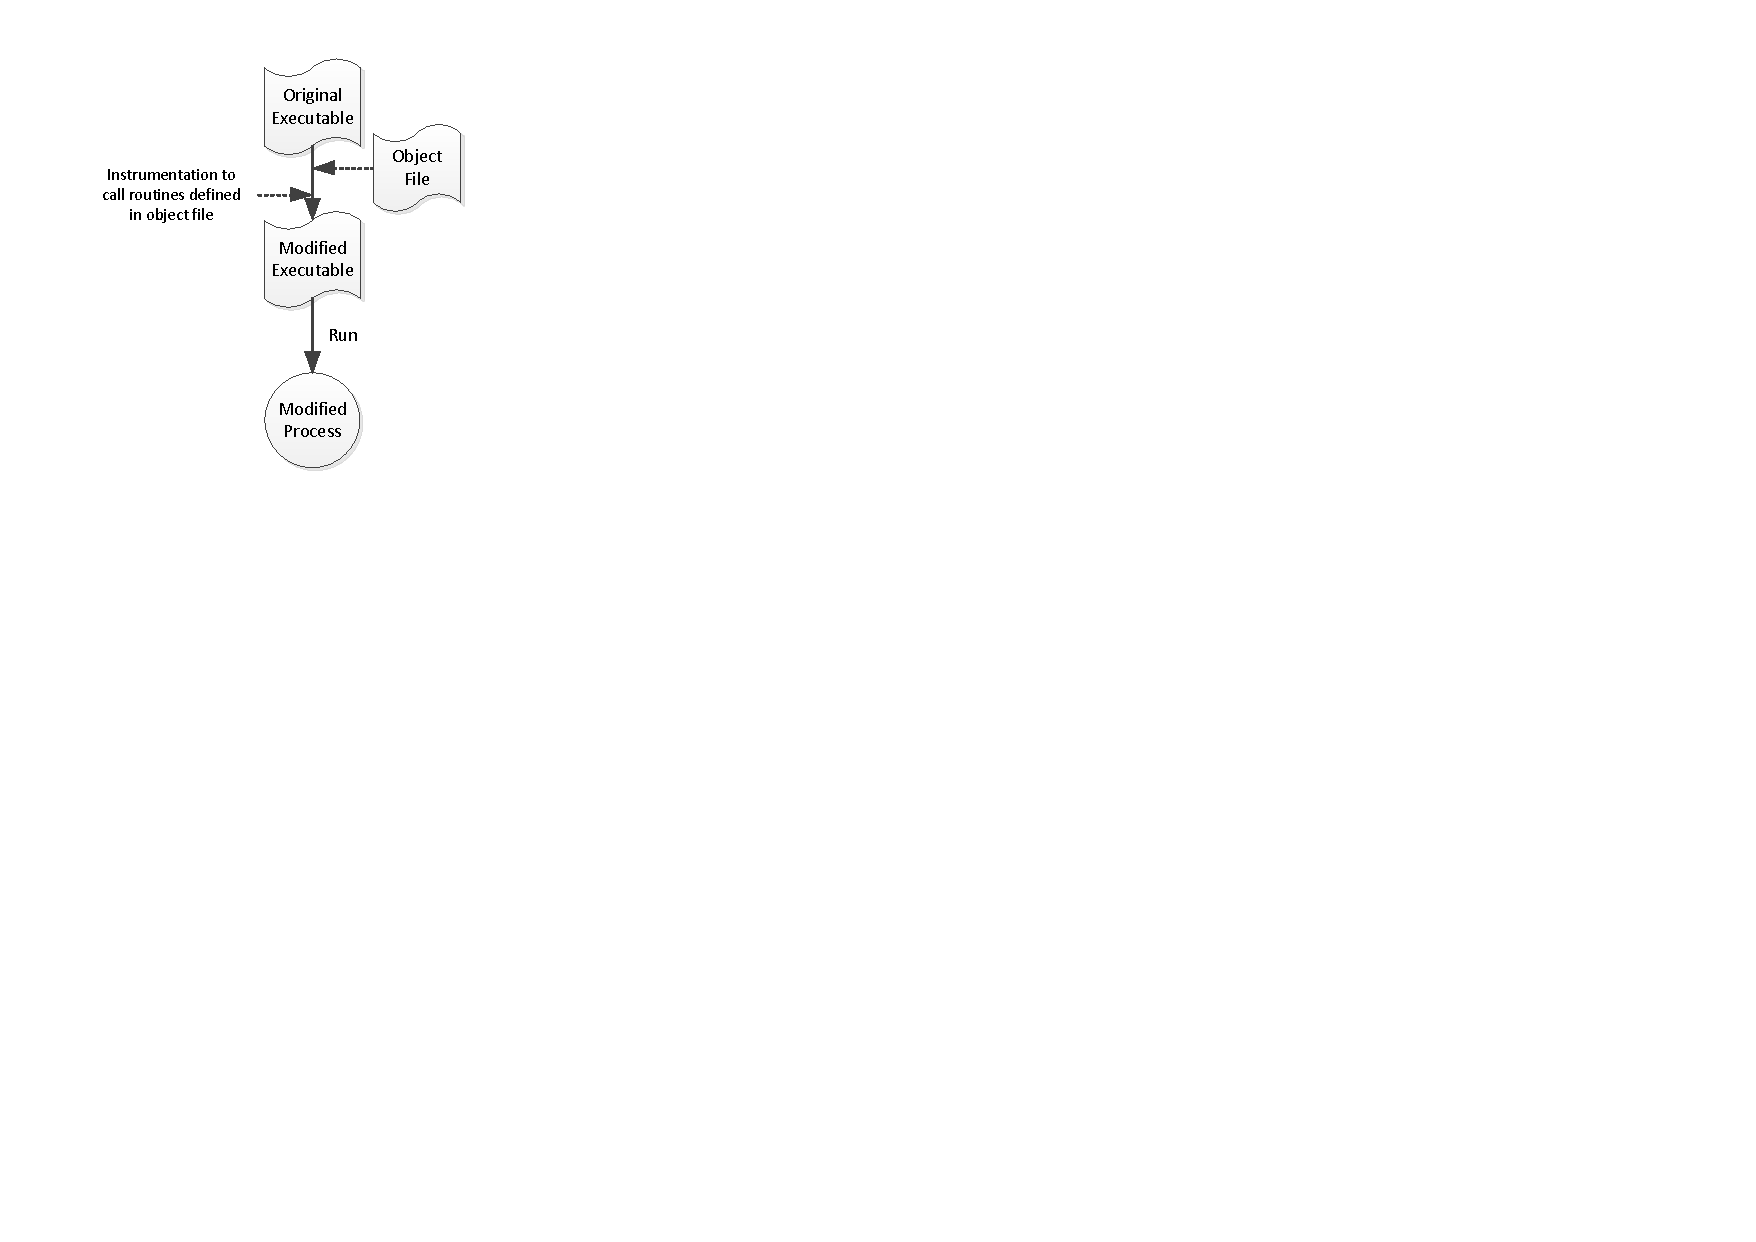
\includegraphics{Workflow.pdf}
 \caption[Hierarchy]{The proposed method for instrumentation. An object file containing user defined routines is optionally injected into the target binary. Using binary rewriting, the original code is then connected to the injected code.}
\label{fig:Workflow}
\end{figure}

from the proposed workflow, it can be seen that there are two distinct phases:

1. object injection which will take original binary + object => binary with user defined routines. satisfies f6.
2. binary rewriting to statically patch detours and trampolines into the binary which contains user defined routines. satisfies f1, f2, f3.

on top of this, we will add one more phase which is a binary analysis stage. we borrow the concept from Etch of having a code discovery stage. this will allow users to select what function or basic block they are going to detour/trampoline. this binary analysis should also produce the cfg that is required by \emph{(F4)} and \emph{(F5)}. in terms of \emph{(F7)}, it is an implicit implementation detail.

\section{Static Analysis Engine}

the static analysis engine corresponds to the binary analysis stage mentioned above. to re-iterate, the aims of the static analysis engine is to generate a cfg from a binary and expose an interface to it. the user then will iterate the discovered basic blocks and functions, choosing one to instrument. providing such functionality will require a disassembler engine.

\subsection{Disassembler Engine}

we could create our own disassembler engine, but that is unnecessary given the number of implementations already existing. it would be convenient to use a disassembler that can disassemble both x86-32 and x86-64. libopcodes is a natural choice because it is distributed as part of gnu binutils, which makes it readily available. furthermore, gnu binutils are ported to many platforms. this means that if it turns out in the future that we want to port our library to another architecture, it is likely we can reuse the disassembler engine. besides portability, one of the reasons using bfd is good is that it abstracts from libelf, which we want to avoid if possible \emph{(F7)}.

unfortunately, libopcodes has several shortcomings:
1. limited to disassembly of a single address (as opposed to disassembling a function, etc.)
2. designed to print to stream (not stored or analyzed)

libopcodes is likely to continue to be supported for the foreseeable future given that widely used binutils tools build on top of it. most notably, objdump. unfortunately, we are unable to make use of objdump because it does not support control-flow disassembly.

this means that in order to generate a cfg, we need to write our own code that generates one from single instructions. furthermore, we need to override the behaviour where it outputs to a stream. there already exists a library, libopdis, which wraps libopcodes to achieve exactly these core functionalities. however, we want a lightweight library so it is not optimal to build on top of libopdis. worse than this is the fact that libopcodes (like many disassemblers) only offers instruction information in terms of strings. string operation is inefficient and inconvenient so if we can find some solution which solves this problem, it would be good. in fact, even libopcodes returns strings when disassembling (it is meant to work with streams after all, so this makes sense). but this means libopcodes is a thin wrapper which should not be difficult to reproduce.

\section{Object File Injection}

...

\section{Static Patcher}

it is convenient that we are going to use bfd for the static analysis engine because it is also possible to write files through bfd. in fact, this is what several well known binutils tools do (e.g. objcopy and ld).

\section{Summary of Design}

We propose an implementation of executable editing which works on top of the BFD library. This makes adaquate use of existing functionality as required by \emph{(F7)}. BFD will work in conjunction with the libopcodes library to produce the control flow graph as required by \emph{(F4)} and \emph{(F5)}. To inject user-defined routines, we can take a similar approach to EEL and allow the user to specify an object file to be merged with the target binary.\todo{...} The next step would then be to find some mechanism by which procedural-level detouring can be achieved \emph{(F1)}, again through BFD. This is the first point at which we are modifying the target's code in any way. The technique used will have to be modified slightly to accommodate for the trampolining as required by \emph{(F2)}. Since the user defined functions are compiled separately to the target, they do not know what address to call for the trampoline so this is something we will have to deal with.